\chapter{Accurate Soft Error Simulation Using Adaptive Partitioning} 

As technology continues to the scale down, the likelihood of a radiation induced error increases. This trend provides a need for accurate and efficient methods to calculate the soft error rate of a given circuit. Since it is expensive and time consuming to design and circuit and test at a later time, efficient tools that can accurately determine the error rate for a given netlist before fabrication can significantly reduce the design time. However, it has proven to be very difficult to characterize combinational circuits due to three pulse masking factors. The masking factors are as follows:

\begin{enumerate}
	\item Logical Masking: The pulse is removed due to the boolean inputs on the gate during pulse generation or a controlling value on an off-input during pulse propagation.
	
	\item Electrical Masking: The first order RLC effects within the gate cause the pulse to degrade and fully attenuate.
	
	\item Temporal Masking: The pulse arrives at a flip-flop but does not meet the set-up and hold time parameters. 
\end{enumerate}

Considering the above factors, all current soft error simulators consist of modeling a particle at a specific energy which is used in an equation to model the error pulse shape \cite{injeq}. Once the pulse is generated, it is propagated through the combinational logic to the output. It is then assumed that the output is connected to a flip-flop thus the set-up and hold times are considered. It has been shown in \cite{MARS_C,METSys} that concurrent estimation of all masking factors is required in order to ensure that the soft error rate is calculated accurately. However, due to limitations on simulation time and available memory, efficient and accurate consideration of all masking factors has proven to be a difficult and ongoing problem. 

There have been many approaches to improve the estimation of the three factors. First the existing approaches to the estimation of logical masking will be discussed. The most common method to calculate the logical masking effects is the use of a Monte Carlo based simulation which consists of randomly applying patterns as in \cite{Accurate_Masking,SERA,SEMM,PARAM_DESC,SETA_LA}. While this approach is very easy to implement, it suffers from accuracy and run time issues when the circuit has more than 30 inputs. In the case of large circuits, the simulator must resort to generating random input patterns which cover only a small subspace of the possible inputs. This implies that the error in logical masking estimation increases with the circuit size. 

To enhance on Monte Carlo based simulation, the authors in \cite{PTM} propose the use of probabilistic transfer matrices (PTM). This approach consists of representing the Boolean functions within a matrix in which Boolean operations can be applied. While being very accurate, the use of PTMs are non-ideal since they have high memory and simulation time costs that explode on small circuits. The authors in \cite{Han2014} propose an enhanced alternative to the PTM method which uses stochastic logic to calculate the signal probabilities for logical masking estimation. While their method is fast, it relies on the use of random input patterns that can limit the accuracy of the calculation.

Another common approach found in \cite{Chen2013,Li2016} uses the correlation coefficient method (CCM) proposed in \cite{Ercolani1989}. This method uses basic gate signal probability functions to determine the output. For example, the probability of an AND gate is given as $P(O) = P(A)P(B)$ where $P(O)$ is the output probability, $P(A)$ is the probability of input $A$ being "1" and $P(B)$ is the probability of inputs $B$ being "1". A drawback with using the basic probability functions is that they are unable to consider the correlations between signals. CCM improves on this by add a correlation factor to estimate the signal probability. While CCM does provide quick estimation of the logical masking effects with virtually no memory overhead, it can only estimate first order correlation. This implies that as the circuit gets larger, the accuracy of the method substantially decreases.

The last approach discussed in this section, which is of most concern in this paper, is the use of binary decision diagrams (BDDs). BDDs provide a very accurate way to determine the logical masking effects since they are a condensed canonical form of a Boolean function. The main problem with BDDs however, is that they scale exponentially with circuit size thus leading to the possibility of blow up on medium to large circuits. Despite this problem, there have been many proposed simulators that the use BDDs \cite{FASER,MARS_C,METSys}. The main advantage to the use of BDDs is that all input patterns can be considered concurrently thus allowing for exact calculation of logical masking probabilities.

To alleviate the inherent blow up problem, the authors in \cite{FASER} propose the use of partitioning. In their work, they show that the use of partitioning allows for much faster calculation of the soft error with no threat of blow up at a cost of accuracy. The authors in \cite{METSys} also investigate partitioning but do not give an in depth study on how partitioning effects the output error. In both approaches, the circuit is partitioned before simulation with each partition size being set to a predetermined value. This is problematic since the size may be much smaller or larger compared to the given time, processing power and memory. For this reason, this section proposes the use of an adaptive partitioning algorithm that scales the partition size based on the number of nodes. It is shown that the adaptive method allows for faster and more accurate estimation of the logical masking effect compared to the non adaptive approach.

In addition to the adaptive partitioning approach, the proposed simulator has the capability of considering multiple concurrent pulse strikes commonly referred to as multiple event transients (METs). The consideration of multiple strikes has become of greater concern due to the small feature size, leading to a lower critical charge for upset, and the closer placement of transistors \cite{Rossi2005}. These type of events can occur in two forms: single event multiple transient (SEMT) and multiple event multiple transient (MEMT). A SEMT is defined as the case where a single radiation particle upsets multiple transistors causing multiple transients pulses. A MEMT is defined as when multiple particles hit different circuit components simultaneously. While the probability of the SEMT vs the MEMT depends strongly on the radiation environment, methods developed for one type of error can easily be modified to consider the other. 

There are a few existing methods that include the consideration of multiple event errors. The authors in \cite{METSys} consider the correlation of METs however their method uses BDDs which tend to blow up. While they do investigate the use of partitioning, their method is only tested for small circuits using only a few concurrent pulses. An additional simulation tool used for MET analysis found in \cite{Fazeli2011} uses probabilistic functions. This approach has shown to be fast and efficient but is not suited for the use of complicated electrical masking methods. The approach proposed in this section applies the pulse approximation method given in Chapter \ref{ch2} to a MET simulation methodology which allows for much more accurate soft error calculation.

\section{Adaptive BDD Based Simulation} 

A crucial aspect in the estimation of the logical masking effects is accurate creation of the Boolean functions. To ensure full consideration of the logical masking effects, Boolean functions must be created to evaluate the circuit inputs for pulse generation and the off-inputs for pulse propagation. First the method to generate the functions for error pulse generation will be discussed. 

When a high energy particle strikes a transistor, the magnitude and polarity of the pulse will depend on the configuration of the transistor. In the case of CMOS logic, a transient pulse is generated when a particle hits a blocking transistor. This will, in turn cause the transistor to temporarily conduct current allowing for the generation of the voltage pulse. In Fig. \ref{NANDS} a 2 input NAND gate is given to demonstrate this mechanism. In the NAND gate, a particle can hit a single PMOS or a NMOS transistor to cause an error. However, since the transistor must be blocking, the input pattern has a large effect on where the error will occur and the polarity of the pulse. 

For example, in the 2 input NAND gate in Fig. \ref{NANDS}, if both inputs have a value of "1", a strike on either of the PMOS transistors will likely cause a transient pulse. In the case of one input having a "0" value and the other a "1" value,  a strike on the blocking NMOS transistor will cause an error. In the case of both inputs having a "1" value, the gate will only generate a transient pulse if both NMOS transistors are struck concurrently. Addition, the polarity of the pulse also requires consideration. If the output is has a "1" value, the pulse will start at a high value, go low and back to a high value. When the output has a "0" the pulse will start at a low value, go high and back to a low value. Based on this observation, the function for the pulse generation for the AND, NAND, OR and NOR are given in Table \ref{table:gentable} for a $N$ number of inputs with each input denoted as $I_i$.

\begin{figure}[!htbp]
	\centering
	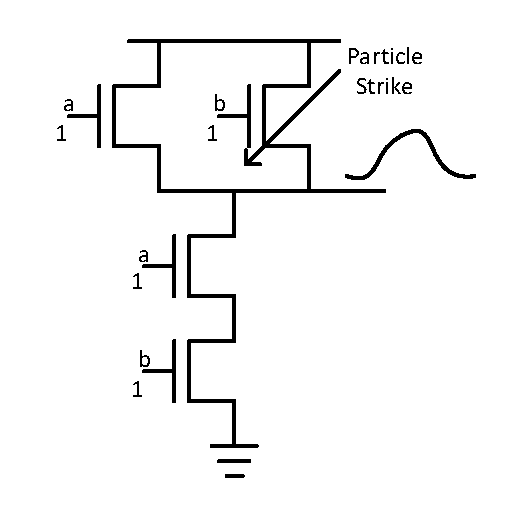
\includegraphics[width=0.55\linewidth]{Figures/NAND_Strike}
	%where an .eps filename suffix will be assumed under latex, 
	%and a .pdf suffix will be assumed for pdflatex; or what has been declared
	%via \DeclareGraphicsExtensions.
	\caption{A low-high-low transient pulse being generated by a strike on the PMOS.}
	\label{NANDS}
\end{figure}

\begin{table}[h]
	\begin{center}
		\caption{Functions for Transient Pulse Generation}
		\label{table:gentable}
		\begin{tabular}{|c|c|c|}
			\hline
			Gate & Polarity & Generation Function ($F(G)$) \\ 
			\hline
			AND & Rising & $F(G) = 1 - \prod_{i=1}^{N} I_i$\\
			\hline
			AND & Falling & $F(G) = \prod_{i=1}^{N} I_i$\\
			\hline
			NAND & Rising & $F(G) = \prod_{i=1}^{N} I_i$ \\
			\hline
			NAND & Falling & $F(G) = 1 - \prod_{i=1}^{N} I_i$ \\
			\hline
			OR & Rising & $F(G) = \prod_{i=1}^{N} \bar{I_i}$ \\
			\hline
			OR & Falling & $F(G) = 1 - \prod_{i=1}^{N} \bar{I_i}$ \\
			\hline
			NOR & Rising & $F(G) = 1 - \prod_{i=1}^{N} \bar{I_i}$ \\
			\hline
			NOR & Falling & $F(G) = \prod_{i=1}^{N} \bar{I_i}$ \\
			\hline
		\end{tabular}
	\end{center}
\end{table}

When a pulse is propagated to the input of gate, the pulse will be masked if one of the off-inputs has a controlling value. Fig. \ref{Prop_NAND} gives a NAND gate with one of the inputs having a pulse and the other input having a controlling "0" value. In this case, the output will be a logical "1" value despite the pulse on the input.

\begin{figure}[!htbp]
	\centering
	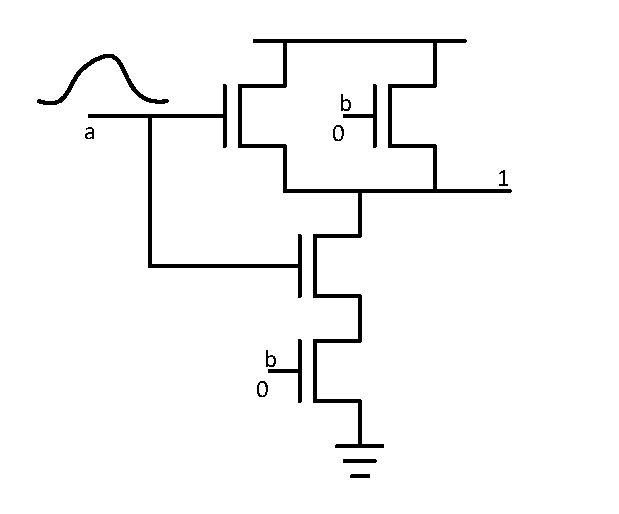
\includegraphics[width=0.55\linewidth]{Figures/Prop_func}
	%where an .eps filename suffix will be assumed under latex, 
	%and a .pdf suffix will be assumed for pdflatex; or what has been declared
	%via \DeclareGraphicsExtensions.
	\caption{A transient pulse being masking by a controlling value on the off-input.}
	\label{Prop_NAND}
\end{figure}

To calculate the logical masking factor during pulse propagation, the functions of the off-inputs are calculated using the logical AND operation. Assume that $P(I_i)$ is the Boolean function of the input $I_i$ and there are a $N$ number of inputs, the function of the probability of the transient pulse being logically masked during propagation $P(M)$ is given below:

\begin{equation} \label{prop_eq}
P(M) = \prod_{i=1}^{N-1} I_i
\end{equation}

In equation \ref{prop_eq} only $N-1$ inputs are considered since the input which contains the transient pulse is not included in the calculation. 

For the consideration of METs, the above equations must be modified such that the joint probability of the error occurring is considered. In the case of pulse generation, it is assumed that a single radiation particle will strike two or more gates causing transient pulses. In the case of pulse generation, the equation for the number of possible ways a strike can produce a pulse ($P_{num}$) is given in equation \ref{num_eq} assuming a $N$ number of struck gates and $r$ as the number of gates that produce a transient pulse.

\begin{equation} \label{num_eq}
P_{num} = \sum_{r=1}^{N} \frac{N!}{(N-r)!}
\end{equation}

Equation \ref{num_eq} is derived based on the fact that multiple pulses can be masked before they arrive on the gate. More specifically, given that NAND gate in Fig. \ref{Prop_NAND}, it is possible for up to two pulse to arrive simultaneously. This arrives to 3 possible cases given in Fig. [ref]. Based off the three cases, the probability of MET occurring is given in equation [ref] where $P(A)$ is the probability of the pulse arriving on input $A$, $\bar{P(A)}$ is the probability of the pulse on input $A$ not arriving and $P(A_{NC})$ is the probability of input $B$ having a non-controlling value. The variables apply to input $B$ similarly.